\documentclass[a1paper, 25pt, colspace=5mm, 
subcolspace=0mm, 
blockverticalspace=5mm, innermargin=5mm]{tikzposter}

\usepackage[rounded]{syntax}
\usepackage{listings}
\usepackage{url}

\title{A language and compiler for game structures}
\author{Brooks MacLachlan}
\institute{McMaster University}
\date{\today}

\usetheme{Desert}

\useblockstyle{Basic}

\usebackgroundstyle{Empty}

\begin{document}
	\maketitle
	\begin{columns}[fragile]
		\column{0.5}
		\block{Background}{\begin{itemize}
				\item A ``game'' is an activity involving some number of 
				players and a way to ``win''
				\begin{itemize}
					\item Ex. sports, reality show games
				\end{itemize}
				\item Infinitely many games are possible, but running most 
				games would require a human ``host''
				\item An easy-to-understand DSL for describing game structures
				and generating programs to run the game could reduce the 
				need for human hosts and eliminate 
				possibility of host biases affecting game results
			\end{itemize}}
		\block{Related Work}{\begin{itemize}
				\item Existing game DSLs are focused on video games or computer 
				players ([1], for example)
				\item Brantsteele is a website for simulating games [2]
				\item Few playable game variations available on websites such 
				as Tengaged [3] and Zwooper [4]
				\item Online Reality Games (ORG) designed and run by human 
				hosts are often played on social media platforms (see [5])
			\end{itemize}}
		\block{Development Information}{\textbf{The Program}
			\begin{itemize}
				\item 1500+ lines of Haskell code
				\item Target language is Python
			\end{itemize}
			\textbf{Documentation}
			\begin{itemize}
				\item All Haskell functions formally documented with Haddock
			\end{itemize}
			\textbf{Tests}
			\begin{itemize}
				\item Parser, PreCompiler, and Compiler are fully unit-tested 
				using the HSpec framework in Haskell
				\item Over 320 test cases in total!
				\item 6 additional full example games act as 
				integration tests
				\begin{itemize}
					\item Tennis, baseball, Survivor, Big Brother, The Genius, 
					original
				\end{itemize}
			\end{itemize}}
		\begin{subcolumns}
			\subcolumn{0.45}
			\block{References}{\small
			$[1]$ Love, N., Hinrichs, T., Haley, D., Schkufza, E., Genesereth, 
			M. (2008). General Game Playing: Game Description Language 
			Specification. \textit{Stanford Logic Group}.\\
			$[2]$ Brantsteele. \url{https://brantsteele.com}\\
			$[3]$ Tengaged. \url{https://tengaged.com}\\
			$[4]$ Zwooper. \url{https://zwooper.com}\\
			$[5]$ OnlineSurvivor. 
			\url{https://www.reddit.com/r/OnlineSurvivor/}}
			\subcolumn{0.55}
			\block{Modules}{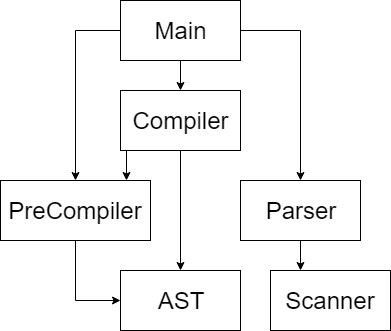
\includegraphics{ModuleHierarchy}}
		\end{subcolumns}
		\column{0.5}
		\block{Subset of the Grammar}{
			\begin{grammar}
				<game> ::= `Players:' <teamList> `Rounds:' <roundList> `Win:' 
				<winCondition>
				
				<competition> ::= [`scored'] [`team'] `competition between' 
				<identifierList>
				
				<decision> ::= `vote by' <identifierList> `between' 
				<identifierList> [`including self'] | ...
				
				<affiliationUpdate> ::= (`add' | `remove') 
				<name> | ...
				
				<counterUpdate> ::= `set' <name> `to' <value> | ...
				
		\end{grammar}}
	\block{Example - DSL to Python}{\textbf{Snippet of game description}:
		\lstinputlisting{exGameDesc.txt}
		\textbf{Parser}: Uses the Parsec library
		\lstinputlisting{exParser.hs}
		\textbf{AST node}:
		\lstinputlisting{exAST.hs}
		\textbf{Compiler}:
		\lstinputlisting{exCompiler.hs}
		\textbf{Final Python code}:
		\lstinputlisting{exPython.py}
	}
	\block{Conclusion and Future Work}{\begin{itemize}
			\item The domain of game structures can be captured by a DSL, 
			including well-known and completely original game structures
			\item The generated code in its current form is not particularly 
			useful, improve with user interface, online-support, additional 
			features such as game advantages, more conditional 
			possibilities within rounds, variable names for phases, rounds, or 
			tiebreakers
		\end{itemize}
	}
	\end{columns}
\end{document}